We create a geometry in which constructions are whatever methods are most effective for replicating objects from trash and natural materials.  In classical geometry many of us learned in school, we are restricted to the use of the compass and straight edge.  Then in the geometry used in computers, everything is reduced to numbers and geometry becomes arithmetic.  But in Action Geoemtry we use the technology available today to make shapes which carry information about the symmetries and scales we will use for common constructions.  

Unlike in school where we learn to construct things at random, in Action Geometry the purpose of all geometric construction is to replicate things made out of trash in the way most beneficial to the people in our community.  So to choose geometric tools we look at what is available and what we can build, and then build up our geometry around that.  

The materials we start out using are cardboard, scrap cloth, bamboo, and high density polyethylene from milk bottles.  We also use some commercial off the shelf parts and tools, as well as all the tools of Geometron.  The Geometron language documented in the earlier chapters can be used to make geometric shapes which can be sent to a laser cutter.  The shapes can also be traced off of a screen with thin paper and a pencil, the paper cut out and laminated, and then used as a physical construction.  Or if you have a paper printer, you can print the file you create with Geometron.   The shape set is shown in one of the figures.   It includes a collection of shapes that all use 3 inches as a reference, and which contain information about the standard symmetries and scales from geometron.  This includes 90 degree, 45 degree, 72 and 36 and 108 degree, 60 and 30 degrees, and the Golden Ratio, square root of two, and square root of three.  Along with a standard Geometron ruler 6 inches in length, this set of shapes forms the basis of our whole construction method. 

These shapes can be used to construct a wide range of shapes very quickly which can replicate, using the plastic parts to create a template from cardboard, which gets cut out and then used to trace out the same pattern again and again.   This is self-replicating geoemetry!  You can imagine a design, lay it out using standard symmetry and scales on any Geometron server, then use that design as a guide to hand construct that same shape once in cardboard, cut it out and copy it.  Also, you can take the text data for the symbol you created on the Geometron server, put that in a public pastebin and share that with another person.  That person can copy the data into their local Geometron server, edit the layout, and then use their copy of the shape set to make their copy of the cardboard template, then use a sharpie and box cutter to replicate again and again.  Note also that this replication is cascading, like a critical nuclear reaction: each copied piece of cardboard is itself a template which can be used to trace out to cut out another copy in more fresh cardboard.  So the Mathematics of this if there is a large swarm of people going into a very large feed of corrugated cardboard is that there can be exponential growth of the number of copies of a cardboard shape for a certain number of generations.  This shows how scaling in a self-replicating economy can do things that are not possible in a consumption/production economy.

We use the simplest possible constructions to achieve any given task.  The first things we build are the ArtBox, which is a self-replicating box of art supplies. The figures show the layout of how you can use just a 6 inch equilateral triangle repeated 10 times in the right layout to make an attractive art purse.  The skin is wrapped in colored duct tape applied from the Tape Snake, also described in the figures.  The box contains the shape set and ruler of Geometron described above and in the figures, box cutters, sharpie markers, scissors, googly eyes, and more clothesline.  With this set of art supplies, all you need is this ArtBox fully loaded with the Tape Snake, and you can transform a feed of corrugated cardboard trash into an output feed of the same box which is then used to make more boxes and so on.  

Note that this ArtBox is made from a combination of the octahedron and tetrahedron.  Using these two is a tool we can repeat again and again for simple design of useful structures with the minimum of complexity to replicate.  Each of these also contains the open brand of Trash Robot, which is rainbow and googly eyes.  Each box has googley eyes and a black duct tape mouth to make a face.  This is a recognizable brand identity, but it belongs to no one.  It is not property.  So it can replicate freely.

Another basic construction from cardboard is the Golden Pyramid, which is shown in two of the Figures.  This can be used as the enclosure for a very wide range of technologies, from battery packs to Raspberry Pi Geometron Servers, to lights, robot controls, or stereo equipment.  It has a 6 inch square base, a 3 inch square top, and each side has the same angles as for the Golden Triangle(72 degrees).

Textile arts are created by finding black cloth from scraps and plain black clothes and sewing on geometric patterns with bright solid rainbow colors of felt or some similar material.  Text are created by starting with a square and removing as little material as possible in as simple as possible layout to depict a letter.  The Geometron Raspberry Pi servers are carried around in black cloth bags with a Raspberry Pi Penrose tile layout as shown in one of the figures and a 6 foot clothesline Trash Tie drawstring.  There are two types of Trash Tie: the six foot clothesline terminated in duct taped ends, and the 18 inch nylon parachute cord section with burned ends.  Small black cloth bags are sewn with small trash ties as draw strings, and these have symbols sewn on them representing the different types of clay icon token described in a later chapter.  Large bags are also used to carry around the printer which makes the clay tokens which go in the bags.  Some figures of the textile are left blank, these are filled in by hand in the illuminated manuscript in physical copies, and shared in person along with the physical textile arts and crafts.


Skeletron is a method of building structures of all kinds for supporting technology as well as building shelters and light industrial infrastructure.  The Trash Pole is a roughly 6 foot long piece of bamboo with quarter inch holes drilled just in from each end as well as in the center of the pole, all wrapped in rainbow colored duct tape from end to end.  These poles can be joined at the ends by tying the smaller Trash Tie(18 inch nylon parachute cord) through the holes and tying a square knot.  With ends joined, we can construct again a wide range of three dimensional geometric structures using basic geometry of tetrahedra, octahedra, and small deviations from those.  These constructions can then be sketched out by hand or via Geometron and shared freely across the Street Network, again forming self-replicating physical geometric construction.  These poles can be used to build useful things, which induces passerby to donate duct tape and go scrounge for more bamboo, and join in the work of assembly, making a swarm just expand potentially very fast, as long as the rate of new contributors is maintained.  This again stresses the importance of building a powerful open brand.  If the extreme rainbowcore aesthetic can be used to get peoples attention, that will make something which spreads in an organic way.  Not viral, as it is not just information in a fixed system, but organically, as a physical thing is being replicated.  The bamboo could be substituted with any other straight object, like broomsticks, fenceposts, harder solid sticks, etc.  This whole scheme can of course also be scaled up and down with any other scale and material of straight thin structural element.  

This type of triangular replicated structure can be very strong and can build up fractal trusses to make huge complex structures both on land and in and on water.  Skeletron forms the basis of a totally decentralized modular construction method.  The sticks can form frames, and to build shelters from rain and wind, plastic bottles can be cut into strips and those stripes woven and laminated into giant plastic sheets which can be affixed to the frames.  This can be combined with cardboard and paper trash and things like polystyrene trash to insulate the structure, to make robust livable shelters which can scale based on our Action Geometry.  To become an artist in this form of construction, you will want to study deeply and practice extensively with all constructions involving tetrahedrons and octahedrons.  Experiment, study, document, share, replicate.  

Because we have a lot of things designed to be hung from Trash Poles using Trash Ties, we also want modular hooks to suspend things from the Trash Poles.  These are the S-Hooks, which are made from a stack of 4 corrugated cardboard cutouts wrapped in rainbow duct tape, with googly eyes for branding.  The construction for this is done using the 3 inch square shape from the basic Action Geometry shape set, and is shown in the figure.  Again, each time an S is cloned, that clone is the template to make more S's, so this part can replicate with an exponential growth if it is fed into the right trash feed with the right group of people in a local Trash Robot swarm.

This chapter describes then a set of objects which we can share in a physical place by a physical Geometron Server.  These can be shared, used, given away, bartered, sold, improved upon, and sent along to other places in the world to seed new swarms.  A Geometron Trash Camp might include any subset of the things described here.  Huge camps might have a whole village of livable shelters made from Skeletron with Trash Sheet, insulation, HVAC systems, power, industrial production machinery, telecom infrastructure, water purification, sanitation, and agriculture, and span a substantial area.  A small camp might just be a Server on a Golden Pyramid, hanging from a dumpster at a truck stop via a Trash Tie, delivering documents over a hotspot on a smart phone.  But whatever tools and materials we use, we can rely on the power of the Geometron geometric language to replicate constructions from community to community via the Street Network so that we can reach all of Humanity who wants to share.

\begin{figure}
	\centering
	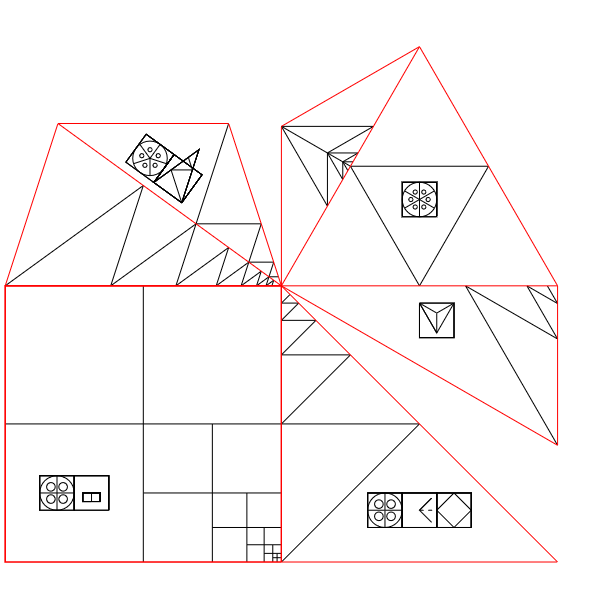
\includegraphics[width=3in]{figures/actiongeometry/shapeset.png}
	\caption[shapeset]
	{Shape Set. This is the basic shape set of Action Geometry.  It has the symmetries and scales of Geometron. What is shown should be printed exactly 6 inches wide, making each shape three inches on a side.}
\end{figure}

\begin{figure}
	\centering
	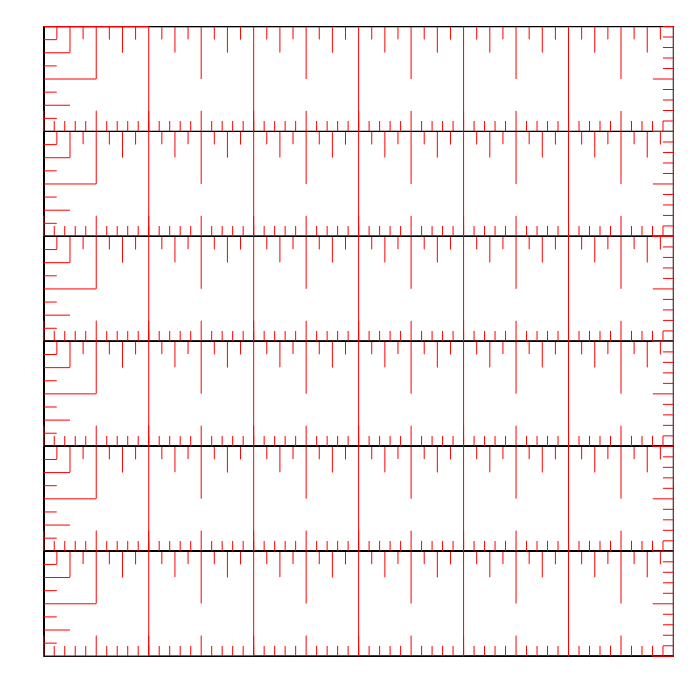
\includegraphics[width=3in]{figures/actiongeometry/rulers.png}
	\caption[rulers]
	{Rulers.  Make this 6 inches wide and each ruler is a 6 inch ruler, 1 inch across, with both tenth and factor of two divisions.}
\end{figure}

\begin{figure}
	\centering
	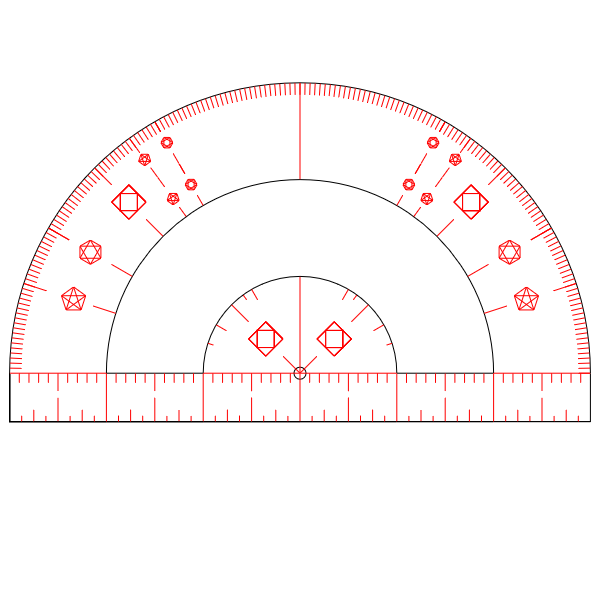
\includegraphics[width=3in]{figures/actiongeometry/protractor.png}
	\caption[protractor]
	{Geometron protractor.  While not really needed for Action Geometry, this protractor is a nice accessory which emphasizes Geometron symmetries rather than numbers, and allows drawing of circles of radius 3,2 and 1 inch without a compass.  This is mostly useful if cut out with a laser cutter.}
\end{figure}


\begin{figure}
	\centering
	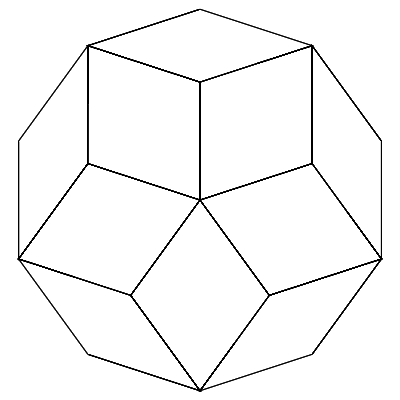
\includegraphics[width=3in]{figures/actiongeometry/penrose.png}
	\caption[penrose]
	{Penrose. Penrose tiles, the rhombi construction.  Copy, print, trace, or laser cut these, and use them to make logos, icons and symbols with some kind of meaning which other people can easily replicate.  The Shape Stack can by copied from someone which has these two shapes, and that can be used to create designs on Servers, which can then also be shared with your community who can all copy your highly recognizable design which has the Trash Robot metabrand as well as whatever symbol you have created or edited.}
\end{figure}

\begin{figure}
	\centering
	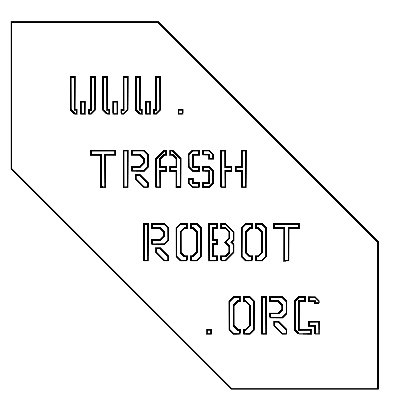
\includegraphics[width=3in]{figures/actiongeometry/stencil.png}
	\caption[stencil]
	{Spray paint stencil for laser cutting. You can use the Geometron software, selecting the built in laser font, to make a custom spray paint stencil pointing to the domain name which points to your Geometron server.  If you are Trash Robot, that can be Trash Robot, but we mostly point to a local non-property place.}
\end{figure}


\begin{figure}
	\centering
	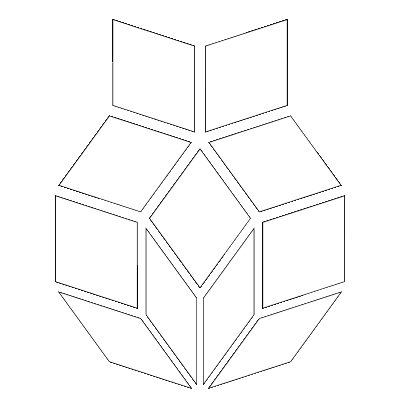
\includegraphics[width=3in]{figures/actiongeometry/pilogo.png}
	\caption[pilogo]
	{Construction of the Raspberry Pi logo for server bags. The top two shapes are green the rest are red.}
\end{figure}


products


\begin{figure}
	\centering
	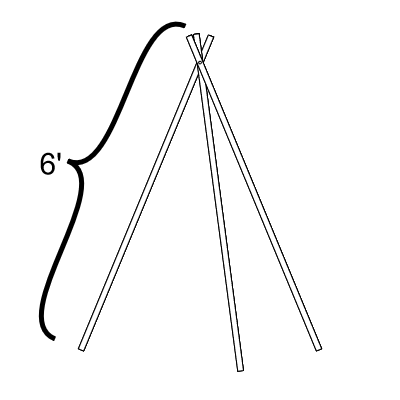
\includegraphics[width=3in]{figures/actiongeometry/skeletrontripod.png}
	\caption[skeletrontripod]
	{Skeletron tripod.  Three 6 foot bamboo trash poles wrapped in rainbow colored duct tape with quarter inch holes drilled just back from the end.  An 18 inch nylon parachute cord trash tie is used with a square knot to secure the top.  Many things can be hung from this, including servers, terminals, robots, boxes, flags, lights, textile arts and pendants on more trash ties.  The tripod can be carried over the shoulder to be mobile, without untying the joint at the top for rapid deployment.}
\end{figure}

\begin{figure}
	\centering
	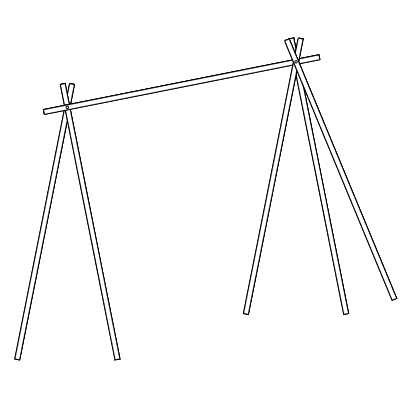
\includegraphics[width=3in]{figures/actiongeometry/skeletron2.png}
	\caption[skeletron2]
	{Skeletron cross bar configuration.  Two tripods can be converted into this stable configuration quickly to have a horizontal cross bar which S-Hooks can hang from to hang numerous objects of all kinds.}
\end{figure}


\begin{figure}
	\centering
	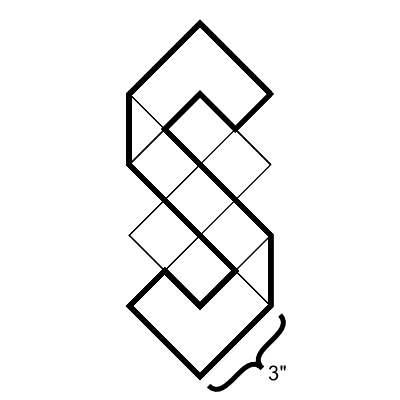
\includegraphics[width=3in]{figures/actiongeometry/shook.png}
	\caption[shook]
	{S-Hook.  Note the repeated use of the square shape, and the use of the 45 degree triangle, making this easy to replicate using the Shape Set.  This hook is used to hang things from the Trash Poles in Skeletron. Fabricate by stacking 4 identical layers of corrugated cardboard cut in this pattern and wrapping them in rainbow colored duct tape.  Googly eyes can then be applied.}
\end{figure}


\begin{figure}
	\centering
	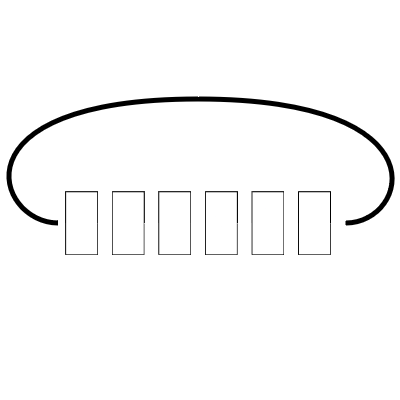
\includegraphics[width=3in]{figures/actiongeometry/tapesnake.png}
	\caption[tapesnake]
	{Tape Snake.  Duct tape rolls of all useful colors, namely the rainbow colors plus black and pink, are strung on a 6 foot Trash Tie made from a clothesline which is looped through twice and secured with a square knot in a bight(like a bow on a tied shoe) for rapid replacement of rolls as they are used.}
\end{figure}


\begin{figure}
	\centering
	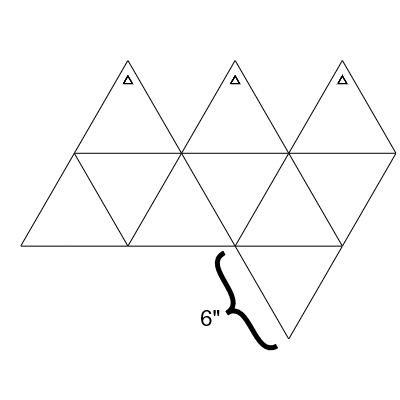
\includegraphics[width=3in]{figures/actiongeometry/artboxnet.png}
	\caption[artboxnet]
	{ArtBox Net.  Cut out 10 equilateral triangles from corrugated cardboard.  Duct tape the joints as shown.}
\end{figure}

\begin{figure}
	\centering
	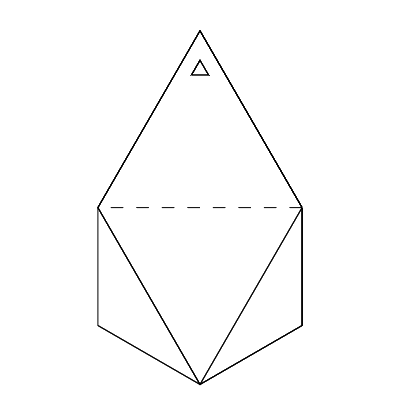
\includegraphics[width=3in]{figures/actiongeometry/artbox.png}
	\caption[artbox]
	{ArtBox assembly.  The fully assembled box is a tetrahedron on an octahedron.  It should contain the means of its own replication, which is a box cutter, a ruler, an equilateral triangle, and a sharpie, along with a Tape Snake for duct tape fabrication, extra Trash Ties, and googly eyes.  Use duct tape colors in sequence to create a fully rainbowed effect, then apply googly eyes and add a black duct tape mouth.}
\end{figure}

\begin{figure}
	\centering
	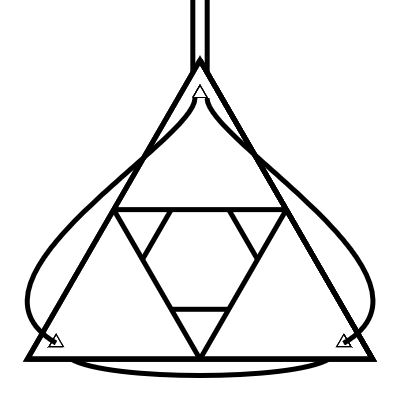
\includegraphics[width=3in]{figures/actiongeometry/artboxtop.png}
	\caption[artboxtop]
	{Top view of ArtBox.  Cut out little triangles in each of the top three petal triangles with the box cutter.  Thread a 6 foot Trash Tie with ends taped with duct tape as shown, and tie off the two bitter ends with a double figure eight knot for convenient purse-strap geometry.}
\end{figure}


\begin{figure}
	\centering
	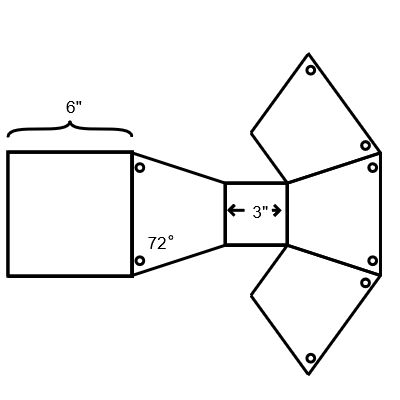
\includegraphics[width=3in]{figures/actiongeometry/pyramidnet.png}
	\caption[pyramidnet]
	{Pyramid net.  Use the Shape Set and Ruler to cut out corrugated cardboard patterns and stitch together with duct tape as shown.  Cutouts include a 6 inch square, a 3 inch square, and four trapezoids with 3 inch top and 6 inch base with 72 degree angles on the bottom angles.}
\end{figure}

\begin{figure}
	\centering
	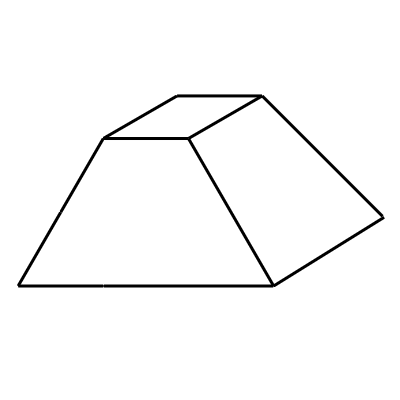
\includegraphics[width=3in]{figures/actiongeometry/pyramid.png}
	\caption[pyramid]
	{Pyramid assembly.  Fold it all up and then cover the whole thing in a skin of rainbow duct tape.  Open the base, insert technology and re-seal.  Add cutouts as needed for cords in and out.}
\end{figure}

\begin{figure}
	\centering
	
\includegraphics[width=3in]{figures/shapes/blank.png}
    \caption[bags]
	{Bags are cut from black cloth, which can be scrap.  Black cloth bags are sewn up with Trash Ties as draw strings.}
\end{figure}


\begin{figure}
	\centering
	
\includegraphics[width=3in]{figures/shapes/blank.png}
    \caption[outfit]
	{Draw your personal Geometron outfit which is black with solid rainbow color felt or similar cloth sewn on in geometric patterns and geometric font.}
\end{figure}
\begin{figure}
	\centering
	
\includegraphics[width=3in]{figures/shapes/blank.png}
    \caption[outfit]
	{Draw your Flag.  A Flag is a black square cloth about 3 feet on a side, with a sewn hem with loops to tie a trash tie.  It is decorated with solid block letters and geometric shapes cut from solid color rainbow felt or similar.  All elements can be from scrap.  Flags point to domains in places.} 
\end{figure}
